\documentclass[10pt,twocolumn,letterpaper]{article}

\usepackage{cvpr}
\usepackage{times}
\usepackage{booktabs}
\usepackage{indentfirst}
\usepackage{epsfig}
\usepackage{float}
\usepackage{amssymb}
\usepackage{amsmath}
\usepackage{picinpar,graphicx}
\usepackage[breaklinks=true,bookmarks=false,colorlinks,
            linkcolor=red,
            anchorcolor=blue,
            citecolor=green,
            backref=page]{hyperref}

\cvprfinalcopy % *** Uncomment this line for the final submission
\def\cvprPaperID{****} % *** Enter the CVPR Paper ID here
\def\httilde{\mbox{\tt\raisebox{-.5ex}{\symbol{126}}}}


\begin{document}

%%%%%%%%% TITLE
\title{Discriminative Region Proposal AdversarialNetworks for High-Quality Image-to-Image Translation}

\author{Wenjie Niu\\\\ July 19,2018}

\maketitle
This writing is also about the paper of \emph{Discriminative Region Proposal Adversarial Networks for High-Quality Image-to-Image Translation}. And this part mainly analyse the method,which I spent 2 days to understand what's the meaning. Therefore, the method is worth considering.
\section{Method}
 Discriminative Region Adversarial Networks(DRPANs) is composed of three components: a generator, a discriminator and a reviser.  The overall network architecture and data flow are illustrated in figure.~\ref{fig:DRPAN}.
 
 \begin{figure*}
 	\begin{center}
 		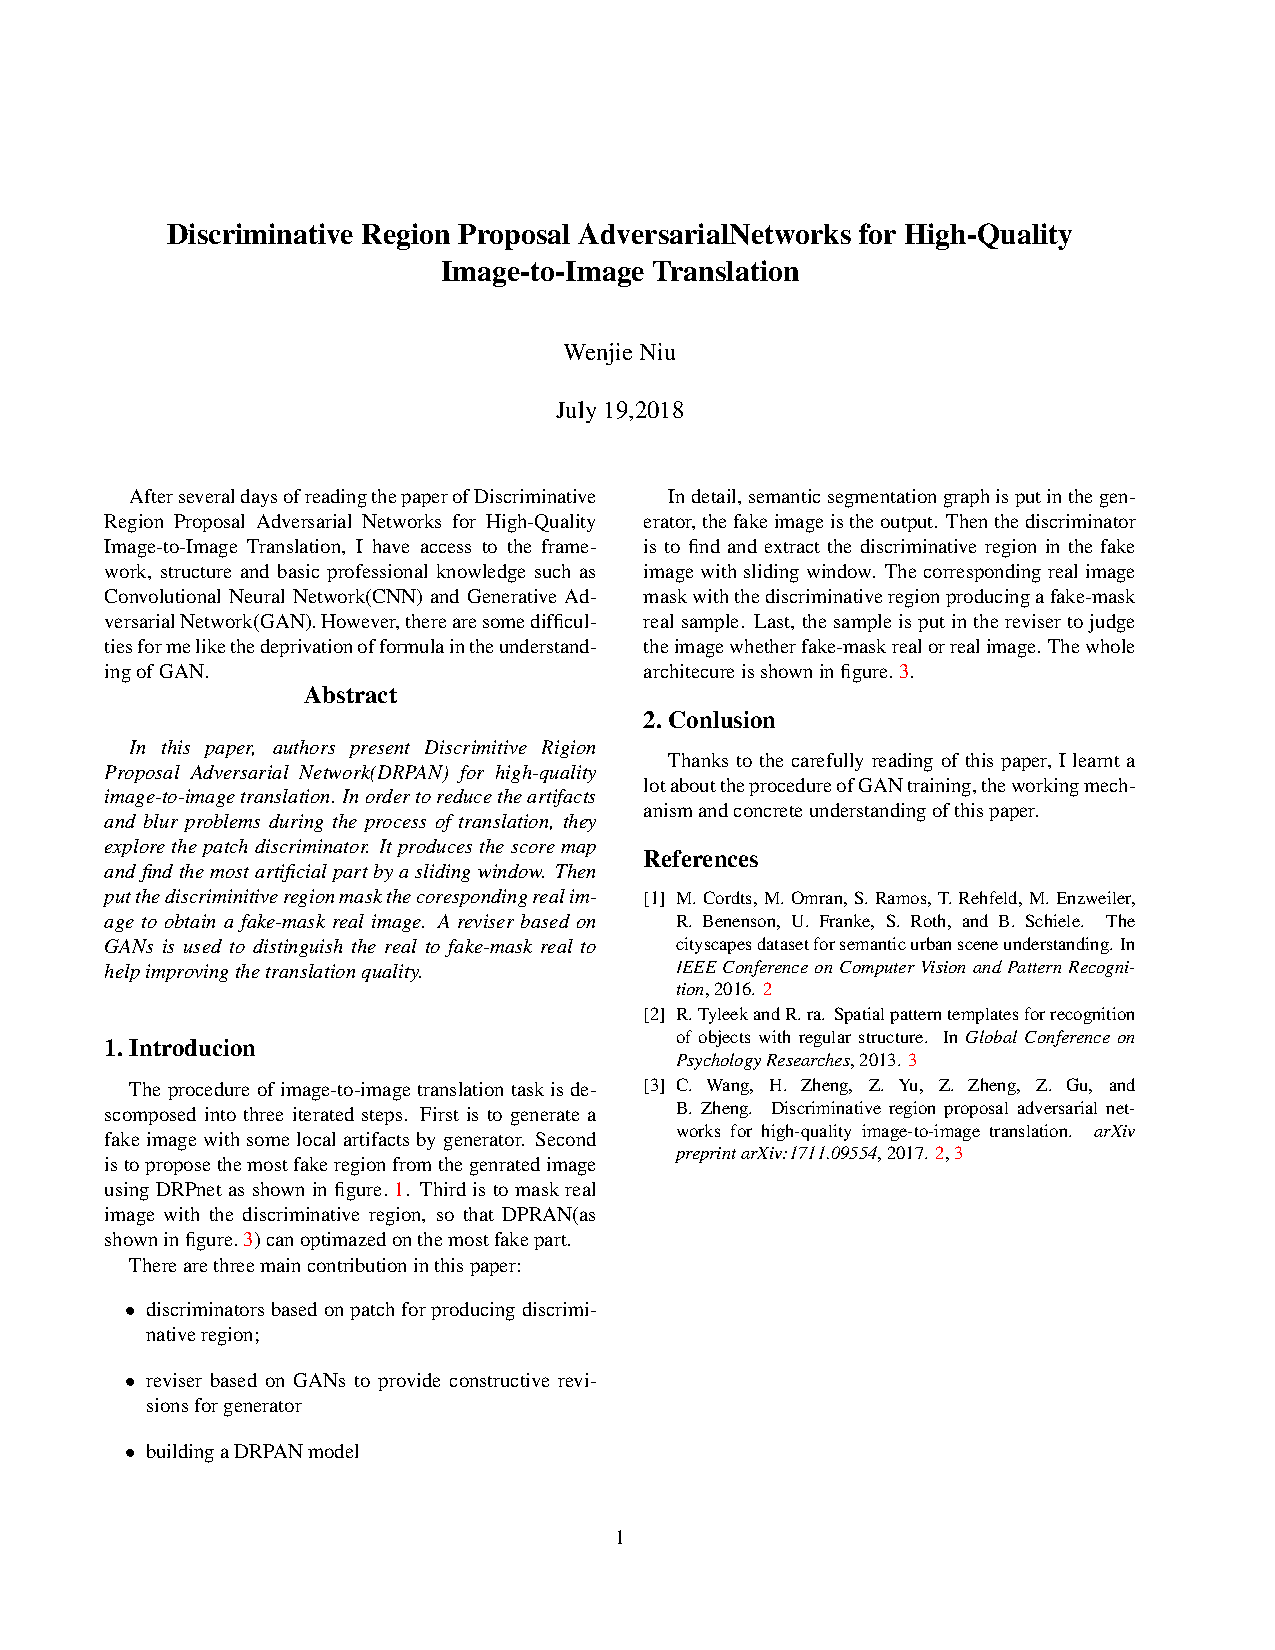
\includegraphics[width=1\linewidth]{DRPAN.png}
 	\end{center}
 	\caption{The overall network architecture and data flow of our proposed Discriminative Region Proposal Adversarial Network (DRPAN), which is composed of three components: a generator, a discriminator, and a reviser, and is a unified model for image-to-image translation tasks~\cite{Wang2017Discriminative}.}
 	\label{fig:DRPAN}
 \end{figure*}
 
  \begin{figure*}
  	\begin{center}
  		\includegraphics[width=1\linewidth]{TrainingProcess.png}
  	\end{center}
  	\caption{The training process of DRPAN on facades dataset~\cite{Radim2013Spatial}. Left: The plotting curve shows mean value of score map on synthesized samples. Right: Step by step synthesis on different discriminative regions~\cite{Wang2017Discriminative}.}
  	\label{fig:TrainingProcess}
  \end{figure*}
  
  \subsection{Objective}
  The original GANs suffer from unstability and mode collapse problem~\cite{Arjovsky2017Wasserstein,Arora2017Generalization}. So some recent works~\cite{Arjovsky2017Wasserstein,Qi2017Loss,Gulrajani2017Improved} improved the training of GAN. To stably train our DRPAN with high-diversity synthesis ability, we modify DRAGAN~\cite{Kodali2017How} as the loss of our reviser $R$, and use the original objective function for training Patch Discriminator.
  \begin{equation}
  \begin{aligned}
  \mathcal{L}_D(G,D_P) = \mathbb{E}_y[logD_P(x,y)]+\\\mathbb{E}_{x,z}[log(1-D_P&(x,G(x,z)))]
  \end{aligned}
  \end{equation}\par
  For reviser R, to distinguish between the very similar real and fake-mask real $y_{mask}=M(G(x,z))$ ($M (·)$ represents the mask operation), they add a regulariza tion to the loss of reviser as the penalty, which is expressed as
  \begin{equation}
  \begin{aligned}
  \mathcal{L}_R(G,R) = \mathbb{E}_y[logR(x,y)]+\mathbb{E}_{x,z}[log(1-R&(x,y_{mask}))]\\+\alpha\mathbb{E}_{x,\sigma}[\lVert\triangledown_xR(x+\sigma)-1\rVert]
  \end{aligned}
  \end{equation}
  where $\alpha$ is hyper parameter, $\sigma$ is random noise on $x$, and $\triangledown$ indicates gradient.\par
  Previous studies have found it beneficial to mix the GAN objective with a more traditional loss, such as L2 and L1 distance~\cite{Isola2016Image,Shrivastava2017Learning}. Considering that L1 distance encourages less blurring than L2~\cite{Isola2016Image}, they provide extra L1 loss for regularization on the whole input image and the local discriminative region to generator, which is defined as
  \begin{equation}
  \begin{aligned}
  \mathcal{L}_{L_1}(G) = \beta\mathbb{E}_(x,y,z)[\lVert y-G(x,z)\rVert_1]+&\\\gamma\mathbb{E}_{d_r,y_r,z}[\lVert y_r-F_{DRPnet}(G(x,z))\rVert_1]
  \end{aligned}
  \end{equation}
  where $\beta$ and $\gamma$ are hyper parameters, $d_r$ is the discriminative region, and $y_r$ represents the region on the real image corresponding to the discriminative region on the synthesized image. Then the total loss of generator can be expressed as
  \begin{equation}
  \begin{aligned}
  \mathcal{L}(G,D_P,R) = -\mathbb{E}_{x,z}[log(1-D_P(x,G(x,z)))]-\\\mathbb{E}_{x,z}[log(1-R(x,y_{mask}))]+\mathcal{L}_{L_1}(G)
  \end{aligned}
  \end{equation}\par
  Their proposed model totally contains a generator $G$, a patch discriminator $D_P$ for DRPnet, and a reviser $R$. $G$ will be optimized by $D_p$ , $R$ and $L_1$ . And our
  full objective function is
  \begin{equation}
  \begin{aligned}
  \mathcal{L}(G,D_P,R) =(1-\lambda)\mathcal{L}_D(G,D_P)+\lambda\mathcal{L}_R(G,R)\\\label{key}+\mathcal{L}_{L_1}(G)
  \end{aligned}
  \end{equation}


\section{Conlusion}
Thanks to the carefully reading of this paper, I learnt a lot about the procedure of GAN training, I understand the method of the paper,which is very strange for me before. The entire procedure is complex and it worth considering again and again.
%-------------------------------------------------------------------------

{\small
\bibliographystyle{ieee}
\bibliography{DRPAN-1}
}

\end{document}
